%!Cau!%
\begin{ex}%[Đề tập huấn, Sở GD - ĐT tỉnh Quảng Bình, 2019]%[Nguyễn Tiến, dự án 12EX5]%[1H2Y1-1]
	Hãy chọn mệnh đề \textbf{đúng} trong các mệnh đề sau.
	\choice
	{\True Nếu một mặt phẳng cắt một trong hai đường thẳng song song thì mặt phẳng đó sẽ cắt đường thẳng còn lại}
	{Hai mặt phẳng lần lượt đi qua hai đường thẳng song song thì cắt nhau theo một giao tuyến song song với một trong hai đường thẳng đó}
	{Nếu một đường thẳng cắt một trong hai đường thẳng song song thì đường thẳng đó sẽ cắt đường thẳng còn lại}
	{Hai mặt phẳng có một điểm chung thì cắt nhau theo một giao tuyến đi qua điểm chung đó}
	\loigiai{
		Ta có tính chất sau: Nếu một mặt phẳng cắt một trong hai đường thẳng song song thì mặt phẳng đó sẽ cắt đường thẳng còn lại.
	}
\end{ex}%!Cau!%
\begin{ex}%[Thi thử L1, Chuyên Lương Thế Vinh Đồng Nai, 2019]%[Nguyễn Tất Thu, dự án(12EX-7)]%[1H2Y1-1]
	Hình chóp ngũ giác có bao nhiêu mặt?
	\choice
	{Bảy}
	{\True Sáu}
	{Năm}
	{Mười}
\loigiai{
Hình chóp ngũ giác có $5$ mặt bên và mặt đáy. Do đó có tất cả $6$ mặt.
}
\end{ex}%!Cau!%
\begin{ex}%[Thi thử, Sở GD và ĐT - Hà Tĩnh, 2019]%[Nguyễn Anh Tuấn, 12-EX8-19]%[1H2Y1-1]
	Hình chóp tam giác có số cạnh là
	\choice
	{$ 3 $}
	{\True $ 6 $}
	{$ 4 $}
	{$ 5 $}
	\loigiai{
		\immini{Xét hình chóp tam giác $ S.ABC $ có các cạnh là $ SA $, $ SB $, $ SC $, $ AB $, $ BC $ và $ CA $. Vậy hình chóp có số cạnh là $ 6 $.}
		{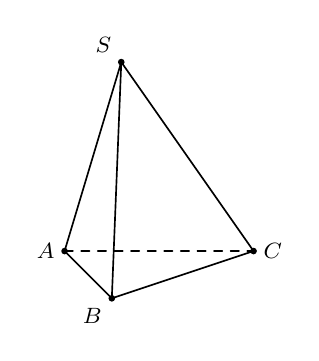
\begin{tikzpicture}[line join=round,line cap=round,line width=.6pt,font=\footnotesize,scale=0.6]
			\coordinate[label=left:$A$] (A) at (0,0);
			\coordinate[label=below left:$B$] (B) at (1,-1);
			\coordinate[label=right:$C$] (C) at (4,0);
			\coordinate[label=above left:$S$] (S) at (1.2,4);
			\draw (A)--(B)--(C)--(S)--cycle (S)--(B);
			\draw[dashed] (A)--(C);
			\fill (A)circle(2pt) (B)circle(2pt) (C)circle(2pt) (S)circle(2pt);
			\end{tikzpicture}
		}
	}
\end{ex}%!Cau!%
\begin{ex}%[Thi thử, Sở GD và ĐT - Hưng Yên-Lần 1, 2019]%[Duong Xuan Loi, 12-EX-8]%[1H2Y1-1]
	Hình chóp tứ giác có tất cả bao nhiêu cạnh?
	\choice
	{\True $8$}
	{$12$}
	{$20$}
	{$6$}
	\loigiai{
		Hình chóp tứ giác có $4$ cạnh bên và $4$ cạnh đáy nên có $8$ cạnh.
	}
\end{ex}